\documentclass[11pt]{article}
\usepackage{xltxtra}
\usepackage{bookmark}
\usepackage{hyperref}
\hypersetup{hidelinks}
\usepackage{url}
\urlstyle{tt}
\usepackage{multicol}
\usepackage{xcolor}
\usepackage{calc}
\usepackage{graphicx}
\usepackage{tikz}
\usetikzlibrary{calc}
\usepackage{fontspec}
\usepackage{xeCJK}
\usepackage{relsize}
\usepackage{xspace}
\usepackage{fontawesome5}
\usepackage{titlesec}
\usepackage{enumitem}
\usepackage{siunitx}
\usepackage{amssymb}
\usepackage{tabularx}
\usepackage{multicol}
\usepackage{fontspec}
\usepackage{fancybox}
\usepackage{float}

% ====================== 基础设置 ======================
% 取消中文字符与数字之间的间隔
\CJKsetecglue{}

% 定义美观的C++排版
\protected\def\Cpp{{C\nolinebreak[4]\hspace{-.05em}\raisebox{.28ex}{\relsize{-1}++}}\xspace}

% 全局格式设置
\setlength{\parindent}{0pt}    % 取消段落缩进
\pagenumbering{gobble}         % 取消页码显示

% 列表格式设置
\setlist[itemize]{topsep=0em, leftmargin=*}    % 项目符号列表格式
\setlist[enumerate]{topsep=0em, leftmargin=*}  % 编号列表格式

% ====================== 标题格式设置 ======================
% 一级标题格式
\titleformat{\section}
  {\LARGE\bfseries\raggedright}  % 字体:LARGE,加粗,左对齐
  {}{0em}                        % 标题前缀
  {}                             % 标题代码
  [{\color{BUPT_Blue}\titlerule}]% 标题下方蓝色分隔线
\titlespacing*{\section}{0cm}{*1.2}{*1.2}  % 间距设置

% 二级标题格式  
\titleformat{\subsection}
  {\large\bfseries\raggedright}  % 字体:large,加粗,左对齐
  {}{0em}                        % 标题前缀
  {}                             % 标题代码
  []
\titlespacing*{\subsection}{0cm}{*1.2}{*1.2}  % 间距设置

% ====================== 页面布局设置 ======================
% 页面尺寸与边距
\usepackage[
    a4paper,
    left=1.2cm,
    right=1.2cm,
    top=1.5cm,
    bottom=1cm,
    nohead
]{geometry}

% 表格与正文行距设置
\renewcommand{\arraystretch}{1.2}  % 表格行距
\linespread{1.2}                   % 正文行距
\renewcommand{\CJKglue}{\hskip 0.05em}  % 中文字符间距

% ====================== 字体设置 ======================
% 英文字体:狮尾四季春
\setmainfont[
    Path=fonts/,
    Extension=.ttf,
    BoldFont=* Bold,
]{SweiSpring}

% 中文字体:狮尾四季春
\setCJKmainfont[
    Path=fonts/,
    Extension=.ttf,
    BoldFont=* Bold,
]{SweiSpring}

% ====================== 主题色设置 ======================
% 北邮校徽标准色(RGB: 0, 51, 153)
\definecolor{BUPT_Blue}{RGB}{0, 51, 153}

% ====================== 个人信息 ======================
% 学院信息
\newcommand{\school}{计算机学院(国家示范性软件学院) | School of Computer Science}

% 联系方式
\newcommand{\contact}{
    \scriptsize  % 使用较小字号
    \textcolor{white}{
        % 邮箱
        \faEnvelope \quad \href{bimu@bupt.edu.cn}{bimu@bupt.edu.cn}
        \hspace{4em}
        % 手机号
        \faPhone \quad  133-0298-4519
        % GitHub
        \hspace{4em}
        \faGithub \quad \href{https://github.com/1BIMU}{https://github.com/1BIMU}
    }
}

%%%%%%%%%%%%%%%%%%%%
% 简历正文
%%%%%%%%%%%%%%%%%%%%
\begin{document}

% ====================== 页眉 ======================
% 包含校徽、学院名称等信息
\begin{tikzpicture}[remember picture, overlay]
    \node[anchor=north, inner sep=0pt](header) at (current page.north){
        
\includegraphics[width=\paperwidth]{images/header.png}
    };
    \node[anchor=west](school_logo) at (header.west){
        \hspace{0.5cm}
        
\includegraphics[width=0.15\textwidth]{images/bupt_logo_name.png}
    };
    \node[anchor=east](school_name) at(header.east){
        \textcolor{white}{\textbf{\school}}
        \hspace{0.5cm}
    };
\end{tikzpicture}
\vspace{-3.5em}

% ====================== 页脚 ======================
% 包含联系方式
\begin{tikzpicture}[remember picture, overlay]
    \node[anchor=south, inner sep=0pt](footer) at (current page.south){
        
\includegraphics[width=\paperwidth]{images/footer.png}
    };
    \node[anchor=center] at(footer.center){\contact};
\end{tikzpicture}

% ====================== 背景 ======================
% 添加校徽水印
\begin{tikzpicture}[remember picture, overlay]
    \node[opacity=0.05] at(current page.center){
        
\includegraphics[width=0.7\paperwidth, keepaspectratio]{images/bupt_logo.png}
    };
\end{tikzpicture}

% ====================== 个人信息 ======================
\begin{figure}[h]
    \begin{minipage}{0.82\textwidth}
        \section{\makebox[\widthof{\faAddressCard}][c]{\color{BUPT_Blue}{\faAddressCard}}\quad 个人信息}
        \begin{tabularx}{\linewidth}{p{\widthof{出生日期:2004-11-10}}Xp{\widthof{政治面貌:共青团员}}X}
            姓\ \ \ \ \ \ \ \ 名: & 王天翼 & 
            性\ \ \ \ \ \ \ \ 别: & 男  \\
            出生年月: & 2004年11月 & 
            政治面貌: & 共青团员 \\
        \end{tabularx}
    \end{minipage}
    \hspace{2em}
    \begin{minipage}{0.12\textwidth}
        \setlength{\fboxsep}{0pt}
        \doublebox{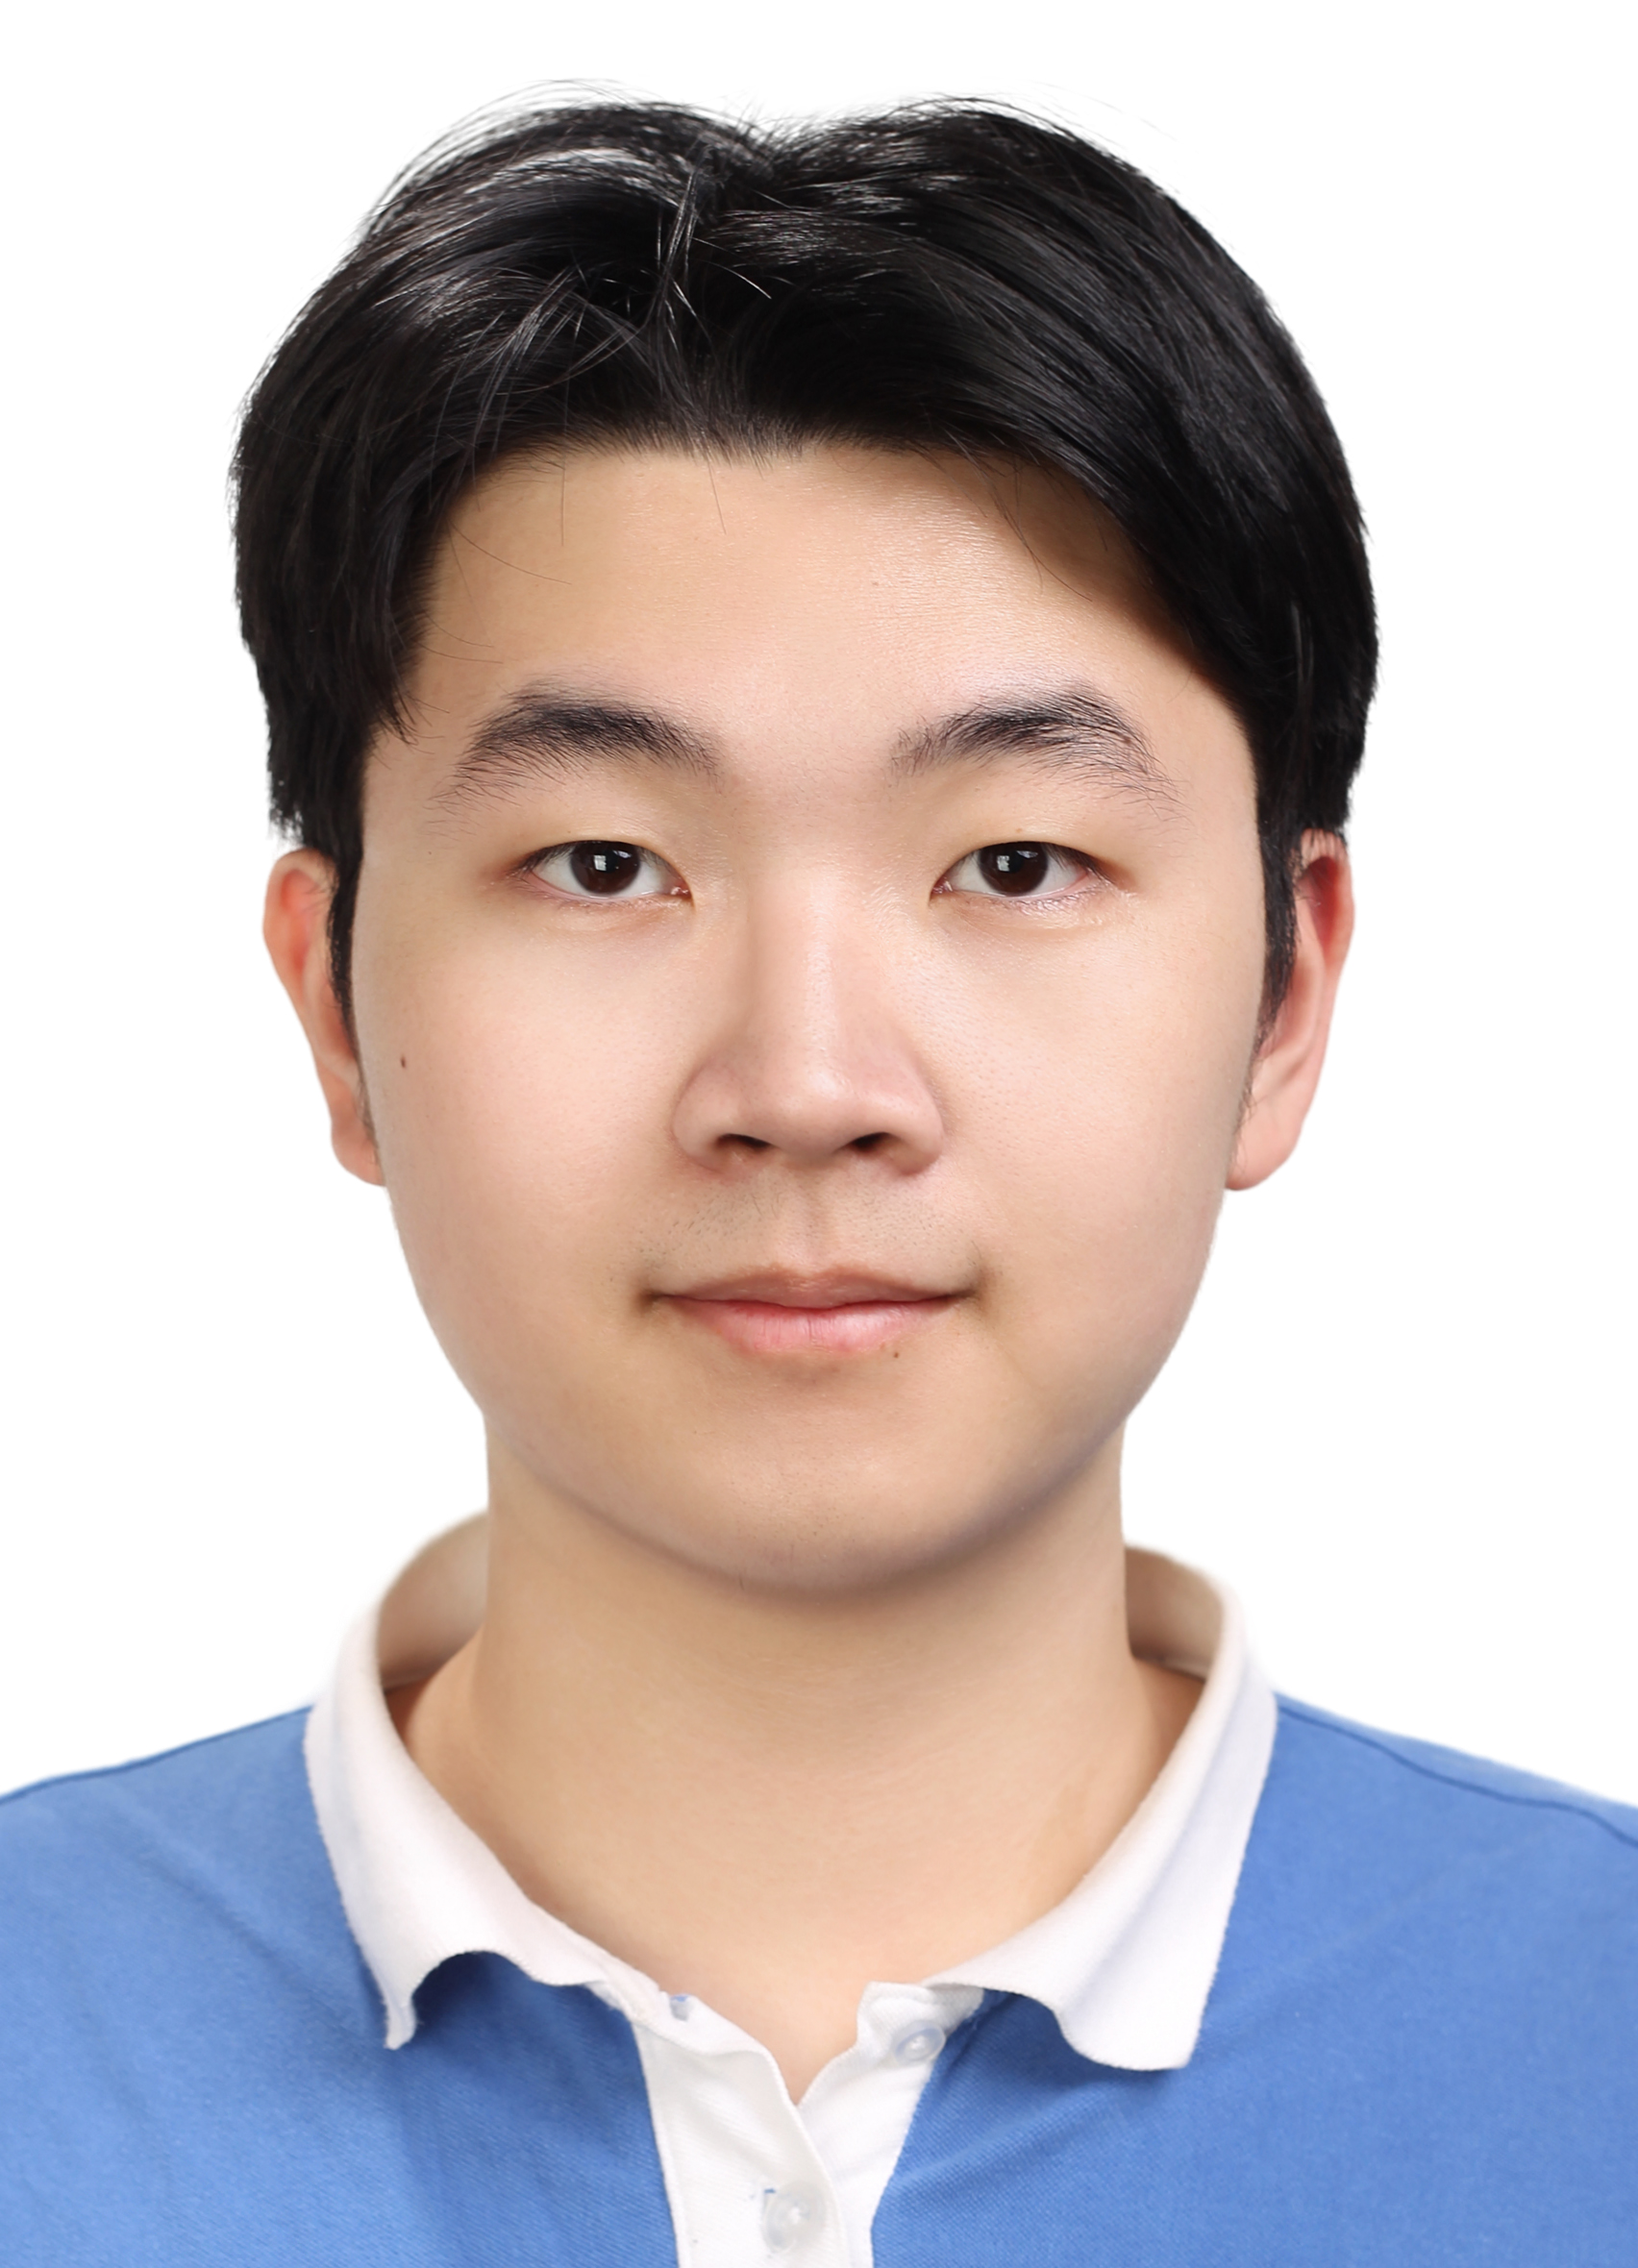
\includegraphics[width=\linewidth]{images/avatar.jpg}}
    \end{minipage}
\end{figure}
\vspace{-1em}

% ====================== 教育背景 ======================
\section{\makebox[\widthof{\faGraduationCap}][c]{\color{BUPT_Blue}{\faGraduationCap}}\quad 教育背景}
\vspace{-0.5em}
\begin{table}[h!]
    \begin{tabularx}{\textwidth}{XXp{\widthof{2023年 -- 预计2027年7月毕业}}}
        北京邮电大学 & 计算机科学与技术 & 毕业年份\ \ \ 2023年 -- 预计2027年7月\\
        \textbf{GPA: 3.75/4.00} & \textbf{GPA排名: 15/480} &\textbf{四级成绩:571}&\textbf{六级成绩:503} \\
    \end{tabularx}
\end{table}
\begin{tabularx}{\textwidth}{@{}XlX@{}}
    \textbf{2023.09-2024.03} & 班级副团支书
\end{tabularx}

% ====================== 项目经历 ======================
\section{\makebox[\widthof{\faChalkboardTeacher}][c]{\color{BUPT_Blue}{\faChalkboardTeacher}}\quad 在校项目}
\vspace{0.5em}
{\large{\textbf{医学影像检测-骨折检测}}} \hfill {完结}\\
是Kaggle上的一个竞赛,主要使用Conv2D卷积神经网络和Dropout正则化,在竞赛的数据集上实现了90±1\%的准确率。

\vspace{1em}
{\large{\textbf{基于LLAMA2的LLM流程}}} \hfill {完结}\\
比较简单的一个对LLAMA2的一个复现,用了自回归,但是没有设置end标记和start标记,因此只能指定长度。使用了SwiGLU激活函数,RoPE编码,Transformer,以及一些其他模块。

\vspace{1em}
{\large{\textbf{LLM自动运维}}} \hfill {进行中}\\
这是一个大模型的应用项目。旨在通过大模型的决策,针对网络上用户的报错进行相关处理。主要使用RAG技术对外部知识库进行检索,并使用LLM进行回答。外部知识库使用爬虫和PDF(运维相关手册)批量导入向量数据库。

% ====================== 科研经历 ======================
\section{\makebox[\widthof{\faFlask}][c]{\color{BUPT_Blue}{\faFlask}}\quad 科研经历}
\vspace{-1em}
\begin{table}[h!]
    \begin{tabularx}{\textwidth}{Xp{\widthof{算法负责人}}p{\widthof{实验室项目}}p{\widthof{2023年9月}}}
        \textbf{基于Qwen2-1.5B的文本分类优化研究} 
        & 算法负责人 & 自研探索 & 2024.12 \\
        \multicolumn{4}{@{}l@{}}{\faCaretRight\ 采用LoRA微调技术,在FudanNews文本数据集上进行了微调} \\
        
        \textbf{深度强化学习算法复现与对比研究} 
        & 算法负责人 & 自研课题 & 2025.03 \\
        \multicolumn{4}{@{}l@{}}{\faCaretRight\ 基于OpenAI Gym构建CartPole实验环境,完成PPO、REINFORCE、Q-learning算法复现} \\
    \end{tabularx}
\end{table}
% ====================== 技能特长 ======================
\section{\makebox[\widthof{\faWrench}][c]{\color{BUPT_Blue}{\faWrench}}\quad 技能特长}
\vspace{0.5em}
\begin{itemize}
    \item 编程语言:熟练掌握Python、C,了解Java
    \item 数据库:熟练使用MySQL
\end{itemize}

% ====================== 所获荣誉 ======================
\section{\makebox[\widthof{\faStar}][c]{\color{BUPT_Blue}{\faStar}}\quad 所获荣誉}
\vspace{0.5em} % 增加正间距
\begin{itemize}
    \item 2023-2024学年三等奖学金
\end{itemize}
\vspace{-0.5em} % 可选:整体列表后轻微回缩

\end{document}
